% Provenance (never printed): see sources/outline_sources.md (Year 3:
% atmospheric dynamics: vorticity and potential vorticity, Rossby waves,
% baroclinic instability, the general circulation and the Hadley cell).
% Brief: sources/book5/BRIEFS.md, ch. 20. Curves from
% figdata/bachelor-3/rossby_waves.py, eady.py and held_hou.py. Exercise and
% problem values in the Book 5 scratch calculator calc/ch20.py. The waves,
% shears and parcels of the exercises and the problem are invented.
\chapter{Dinâmica atmosférica}\label{ch:b3:atmospheric-dynamics}

Em um mapa de inverno da troposfera superior, a corrente de jato não circunda o
polo como um anel liso. Ela serpenteia, em poucas ondas grandes ao redor do
hemisfério, com cavados avançando em direção aos subtrópicos e cristas em direção
ao polo, e na superfície surgem depressões que crescem por alguns dias e se
dissipam sob elas. As ondas se deslocam lentamente, às vezes contra o vento que as
carrega. Seu número, sua velocidade e o crescimento das tempestades abaixo delas
decorrem de uma grandeza conservada, a vorticidade do ar vista do
espaço, e da energia armazenada no contraste de temperatura entre os
trópicos e os polos.

\begin{recall}
Vorticidade e circulação são tratadas nos livros de física. As ondas de Rossby da
troposfera superior, cavados e cristas, o ciclone extratropical e o
princípio da previsão numérica do tempo são descritos no volume do segundo
ano, em seu capítulo sobre sistemas meteorológicos. As células de Hadley, de Ferrel e polar,
os jatos, os ventos de oeste e o vento de momento angular de um anel de
ar estão no volume do primeiro ano, em seu capítulo sobre a circulação geral da
atmosfera, e o transporte meridional de calor em seu capítulo sobre
radiação e transporte de calor. O parâmetro de Coriolis $f$, o plano $\beta$,
o raio de Rossby e o \omterm{thm:b3:gfd-foundations:thermal-wind}{vento térmico} estão no
Capítulo~\ref{ch:b3:gfd-foundations}.
\end{recall}

\section{Vorticidade}\label{sec:b3:atmospheric-dynamics:vorticity}

A vorticidade de um fluido, o rotacional de sua velocidade, é igual ao dobro de sua
velocidade angular local. Para a atmosfera em grande escala, apenas sua componente
vertical importa, e a rotação da Terra contribui para ela.

\begin{definition}[Vorticidade relativa, planetária e absoluta]\label{def:b3:atmospheric-dynamics:vorticity-kinds}
Para uma velocidade horizontal $(u, v)$, a \emph{vorticidade
relativa}\index{vorticidade relativa} é a componente vertical do rotacional
da velocidade em relação ao solo, $\zeta = \partial v/\partial x -
\partial u/\partial y$, positiva para rotação anti-horária vista de cima.
A \emph{vorticidade planetária}\index{vorticidade planetária} é a componente
vertical da vorticidade da rotação da Terra, $2\Omega\sin\varphi =
f$. A \emph{vorticidade absoluta}\index{vorticidade absoluta} é a soma delas,
$\zeta + f$.
\end{definition}

No Hemisfério Norte, uma depressão, onde o ar gira no sentido anti-horário,
tem $\zeta > 0$ e é chamada ciclônica; um anticiclone tem $\zeta < 0$. Um
vento de \qty{15}{m/s} girando em um círculo de \qty{1000}{km} tem $\zeta =
2V/R = \qty{3e-5}{s^{-1}}$ em rotação de corpo rígido, um terço de $f$ a \ang{45}:
a parte planetária costuma ser a maior.

\begin{theorem}[Equação da vorticidade barotrópica]\label{thm:b3:atmospheric-dynamics:bve}
Em um escoamento bidimensional, não viscoso e sem divergência horizontal sobre um
plano $\beta$, a \omterm{def:b3:atmospheric-dynamics:vorticity-kinds}{vorticidade absoluta} de cada parcela é conservada:
\[
\frac{\mathrm D(\zeta + f)}{\mathrm Dt} = 0 ,
\qquad\text{ou seja}\qquad
\frac{\partial\zeta}{\partial t} + u\frac{\partial\zeta}{\partial x} + v\frac{\partial\zeta}{\partial y} + \beta v = 0 .
\]
Esta é a \emph{equação da vorticidade barotrópica}\index{equação da vorticidade barotrópica}.
\end{theorem}

\begin{proof}
As equações horizontais do momento são $\mathrm Du/\mathrm Dt - fv =
-(1/\rho_0)\partial p/\partial x$ e $\mathrm Dv/\mathrm Dt + fu =
-(1/\rho_0)\partial p/\partial y$. Deriva-se a segunda em relação a
$x$, a primeira em relação a $y$, e subtrai-se: a pressão desaparece.
Com $\delta = \partial u/\partial x + \partial v/\partial y$, os termos
advectivos dão $\partial_x(u\,\partial_xv + v\,\partial_yv) -
\partial_y(u\,\partial_xu + v\,\partial_yu) = u\,\partial_x\zeta +
v\,\partial_y\zeta + \zeta\delta$, e os termos de Coriolis, $f\delta + \beta
v$. Logo $\mathrm D\zeta/\mathrm Dt + \beta v = -(\zeta + f)\,\delta$. Para
$\delta = 0$, e como $\mathrm Df/\mathrm Dt = \beta v$, obtém-se $\mathrm D(\zeta +
f)/\mathrm Dt = 0$.
\end{proof}

A demonstração também forneceu a lei geral, $\mathrm D(\zeta + f)/\mathrm Dt =
-(\zeta + f)\delta$: a convergência faz a coluna girar mais depressa, a divergência a
faz girar mais devagar, como uma patinadora que recolhe ou abre os braços. Em uma
camada cuja espessura varia, a convergência está ligada ao estiramento da coluna,
e a grandeza conservada passa a ser uma razão.

\begin{definition}[Vorticidade potencial]\label{def:b3:atmospheric-dynamics:pv}
A \emph{vorticidade potencial}\index{vorticidade potencial} de uma coluna de uma
camada homogênea de espessura $h$ é $q = (\zeta + f)/h$. Em um fluido continuamente
estratificado, a vorticidade potencial de Ertel é $q = (\vec\omega_a\cdot
\nabla\theta)/\rho$, com $\vec\omega_a$ o vetor \omterm{def:b3:atmospheric-dynamics:vorticity-kinds}{vorticidade absoluta} e
$\theta$ a temperatura potencial.
\end{definition}

\begin{theorem}[Conservação da vorticidade potencial]\label{thm:b3:atmospheric-dynamics:pv}
Em uma camada homogênea, hidrostática e não viscosa, de espessura variável $h$, cuja
velocidade horizontal não varia com a altura, $\mathrm Dq/\mathrm Dt = 0$
para $q = (\zeta + f)/h$.
\end{theorem}

\begin{proof}
Pela demonstração anterior, $\mathrm D(\zeta + f)/\mathrm Dt = -(\zeta + f)\delta$.
A conservação da massa em uma coluna de densidade uniforme dá $\mathrm Dh/\mathrm
Dt = -h\delta$. Então $\mathrm Dq/\mathrm Dt = (1/h)\,\mathrm D(\zeta +
f)/\mathrm Dt - ((\zeta + f)/h^2)\,\mathrm Dh/\mathrm Dt = -(\zeta +
f)\delta/h + (\zeta + f)\delta/h = 0$.
\end{proof}

A forma de Ertel se conserva do mesmo modo em um escoamento adiabático e sem atrito
de um fluido estratificado, com a distância entre duas superfícies de
$\theta$ constante fazendo o papel de $h$. Uma coluna de ar que atravessa uma
cadeia de montanhas é comprimida na subida: sua \omterm{def:b3:atmospheric-dynamics:vorticity-kinds}{vorticidade absoluta} diminui, ela
gira anticiclonicamente sobre o topo, e se estica e gira
ciclonicamente a sotavento. A conservação da
\omterm{def:b3:atmospheric-dynamics:vorticity-kinds}{vorticidade absoluta} ou potencial é o mecanismo restaurador das ondas
da próxima seção, como mostra a figura abaixo.

\begin{omfigure}
\begin{tikzpicture}[>=stealth, font=\small, declare function={w(\x)=0.9*sin(\x r);}]
\draw[black!40, dashed] (0,0) -- (12.6,0) node[right, font=\scriptsize] {latitude $\varphi_0$};
\draw[thick, omDef, domain=0:12.566, samples=120] plot (\x, {w(\x)});
\foreach \x in {0.785, 2.356, 3.927, 5.498, 7.069, 8.639, 10.21, 11.78}
  \fill (\x, {w(\x)}) circle (0.06);
% crests: clockwise (anticyclonic), troughs: anticlockwise (cyclonic)
\foreach \x in {1.571, 7.854} {
  \draw[->, omThm, thick] (\x+0.45,{w(\x)+0.05}) arc (0:-300:0.45);
  \node[font=\scriptsize, omThm] at (\x,{w(\x)+0.75}) {$\zeta < 0$};}
\foreach \x in {4.712, 10.996} {
  \draw[->, omMeth, thick] (\x+0.45,{w(\x)-0.05}) arc (0:300:0.45);
  \node[font=\scriptsize, omMeth] at (\x,{w(\x)-0.75}) {$\zeta > 0$};}
\foreach \x in {3.1416, 9.4248} \draw[->, very thick] (\x,0.45) -- (\x,-0.45);
\foreach \x in {6.2832} \draw[->, very thick] (\x,-0.45) -- (\x,0.45);
\draw[->, thick] (8.4,-2.25) -- (6.4,-2.25) node[left, font=\scriptsize] {o padrão se desloca para oeste};
\draw[->] (0,-2.25) -- (1.4,-2.25) node[right, font=\scriptsize] {leste};
\draw[->] (0,-2.25) -- (0,-1.65) node[above, font=\scriptsize] {norte};
\end{tikzpicture}

\par\smallskip{\small Como se desloca uma onda de Rossby (esquema, Hemisfério
Norte). Uma cadeia de parcelas em repouso na latitude $\varphi_0$ é
deslocada até formar uma onda. Mantendo-se $\zeta + f$, as parcelas
deslocadas para o norte, onde $f$ é maior, adquirem \omterm{def:b3:atmospheric-dynamics:vorticity-kinds}{vorticidade relativa}
horária; as deslocadas para o sul, anti-horária. Entre uma crista e o cavado
a leste dela o escoamento induzido é dirigido para o sul; entre um cavado e a
crista a leste dele, para o norte (setas pretas): o deslocamento cresce a
oeste de cada crista e todo o padrão se desloca para oeste.}\label{fig:b3:atmospheric-dynamics:restoring}
\end{omfigure}

\section{Ondas de Rossby}\label{sec:b3:atmospheric-dynamics:rossby}

O volume do segundo ano descreveu as ondas de Rossby da alta troposfera. A
\omterm{thm:b3:atmospheric-dynamics:bve}{equação da vorticidade barotrópica} as explica. Escreva-se o escoamento como um
oeste uniforme $U$ mais uma pequena perturbação com função de corrente $\psi'$,
de modo que $u' = -\partial\psi'/\partial y$, $v' = \partial\psi'/\partial x$ e $\zeta'
= \nabla^2\psi'$.

\begin{theorem}[Dispersão das ondas de Rossby]\label{thm:b3:atmospheric-dynamics:rossby}
Pequenas perturbações $\psi' \propto \mathrm e^{\mathrm i(kx + ly - \omega t)}$
de um vento de oeste uniforme $U$ sobre um plano $\beta$ obedecem à
\emph{relação de dispersão das ondas de Rossby}\index{relação de dispersão das ondas de Rossby}
\[
\omega = Uk - \frac{\beta k}{k^2 + l^2} .
\]
Sua velocidade de fase para leste é $c = \omega/k = U - \beta/K^2$, com $K^2 =
k^2 + l^2$, e sua velocidade de grupo para leste é $c_g = \partial\omega/\partial
k = U + \beta(k^2 - l^2)/K^4$.
\end{theorem}

\begin{proof}
Linearizada em torno de $U$, a \omterm{thm:b3:atmospheric-dynamics:bve}{equação da vorticidade barotrópica} se escreve
$(\partial_t + U\partial_x)\nabla^2\psi' + \beta\,\partial_x\psi' = 0$, desprezando-se
os produtos de quantidades pequenas e sendo nula a $\zeta$ do escoamento básico.
Para a onda plana, $\partial_t \to -\mathrm i\omega$,
$\partial_x \to \mathrm ik$ e $\nabla^2 \to -K^2$: $(-\mathrm i\omega +
\mathrm iUk)(-K^2) + \mathrm i\beta k = 0$, ou seja, $(\omega - Uk)K^2 =
-\beta k$. Derivando-se $\omega$ em relação a $k$ obtém-se $c_g = U -
\beta/K^2 + 2\beta k^2/K^4$, que é a forma enunciada.
\end{proof}

\begin{omfigure}
\begin{tikzpicture}
\begin{groupplot}[group style={group size=2 by 1, horizontal sep=1.7cm},
  width=0.48\linewidth, height=0.46\linewidth, tick label style={font=\scriptsize},
  label style={font=\small}, legend style={font=\scriptsize, draw=none, fill=none}]
\nextgroupplot[xlabel={número de onda zonal $n$}, ylabel={velocidade (\unit{m/s})},
  xmin=1, xmax=12, ymin=-40, ymax=60, legend pos=north east, legend cell align=left,
  title={\small \ang{45} N}]
% computed in figdata/bachelor-3/rossby_waves.py
\addplot[omThm, thick] table[x=n, y=c15] {figdata/out/bachelor-3-rossby_waves-disp.dat};
\addlegendentry{$c$, $U = 15$}
\addplot[omThm, thick, densely dashed] table[x=n, y=cg15] {figdata/out/bachelor-3-rossby_waves-disp.dat};
\addlegendentry{$c_g$, $U = 15$}
\addplot[omDef, thick] table[x=n, y=c0] {figdata/out/bachelor-3-rossby_waves-disp.dat};
\addlegendentry{$c$, $U = 0$}
\addplot[omDef, thick, densely dashed] table[x=n, y=cg0] {figdata/out/bachelor-3-rossby_waves-disp.dat};
\addlegendentry{$c_g$, $U = 0$}
\addplot[black!50, thin, domain=1:12, samples=2, forget plot] {0};
\nextgroupplot[xlabel={latitude (\unit{\degree} N)}, ylabel={número de onda estacionário $n_s$},
  xmin=20, xmax=75, ymin=0, ymax=9, legend pos=north east, legend cell align=left]
\addplot[omMeth, thick] table[x=lat, y=n10] {figdata/out/bachelor-3-rossby_waves-stat.dat};
\addplot[omDef, thick] table[x=lat, y=n15] {figdata/out/bachelor-3-rossby_waves-stat.dat};
\addplot[omThm, thick] table[x=lat, y=n20] {figdata/out/bachelor-3-rossby_waves-stat.dat};
\addplot[black, only marks, mark=*, mark size=1.1pt] table[x=lat, y=ns] {figdata/out/bachelor-3-rossby_waves-statobs.dat};
\legend{\qty{10}{m/s}, \qty{15}{m/s}, \qty{20}{m/s}, janeiro \qty{300}{hPa}}
\end{groupplot}
\end{tikzpicture}

\par\smallskip{\small À esquerda, a velocidade de fase para leste $c$ (contínua) e a
velocidade de grupo $c_g$ (tracejada) das ondas de Rossby com $l = 0$ a
\ang{45} N, em função do número de ondas ao longo do círculo de latitude, sem
vento médio (azul) e em um vento de oeste de \qty{15}{m/s} (vermelho): ondas longas se
deslocam para oeste, ondas curtas são arrastadas para leste, e $c_g > c$. À
direita, o número de onda estacionário para ventos de oeste uniformes de 10, 15
e \qty{20}{m/s}, e para o vento médio zonal de janeiro a \qty{300}{hPa} em cada
latitude (pontos, NCEP--NCAR Reanalysis~1, 1991--2020).}\label{fig:b3:atmospheric-dynamics:rossby}
\end{omfigure}
% ledger: data:b5-ncep-uwnd, geod5:grs80-defining, earth:Rmean

Em relação ao ar, as ondas sempre se deslocam para oeste, tanto mais depressa quanto mais longas
forem. Um vento de oeste arrasta as ondas curtas para leste; as longas ele
não consegue arrastar, e elas derivam para oeste contra o vento. Entre
os dois casos, um comprimento permanece parado.

\begin{proposition}[Ondas de Rossby estacionárias]\label{prop:b3:atmospheric-dynamics:stationary}
Em um vento de oeste $U > 0$, uma onda sem estrutura meridional ($l = 0$) é
estacionária quando seu comprimento de onda é o \emph{comprimento de onda
estacionário de Rossby}\index{comprimento de onda estacionário de Rossby} $\lambda_s =
2\pi\sqrt{U/\beta}$. Ao longo do círculo de latitude $\varphi$, isso corresponde a um
número inteiro de ondas próximo de $n_s = \sqrt{2\Omega a\cos^3\varphi/U}$.
\end{proposition}

\begin{proof}
$c = 0$ quando $k^2 = \beta/U$, logo $\lambda_s = 2\pi/k = 2\pi\sqrt{U/\beta}$.
O círculo tem comprimento $2\pi a\cos\varphi$, logo $n_s = a\cos\varphi\,k =
a\cos\varphi\sqrt{2\Omega\cos\varphi/(aU)} = \sqrt{2\Omega a\cos^3\varphi/U}$.
\end{proof}

A \ang{45} N, em um vento de oeste de \qty{15}{m/s}, com $\beta =
\qty{1.62e-11}{m^{-1}.s^{-1}}$, tem-se $\lambda_s = \qty{6050}{km}$ e $n_s =
4.7$: quatro ou cinco ondas ao redor do hemisfério. Com o vento médio zonal
de janeiro em \qty{300}{hPa}, de cerca de \qty{21}{m/s} a \ang{45} N, $n_s$ fica
em torno de quatro entre \ang{35} e \ang{55} N, diminuindo em direção ao polo. A velocidade de grupo
de uma onda com $l = 0$ excede sua velocidade de fase em $2\beta/k^2$: a energia caminha
à frente da onda, de modo que uma perturbação iniciada em um lugar forma novos cavados
e cristas a jusante dele, alguns dias depois e milhares de quilômetros
a leste, enquanto o padrão em si quase não se desloca. Cadeias de montanhas e os contrastes
de temperatura entre continentes e oceanos forçam ondas estacionárias exatamente
deste tipo, por meio do alongamento e da compressão da
\omterm{def:b3:atmospheric-dynamics:pv}{vorticidade potencial}.
% ledger: geod5:grs80-defining, earth:Rmean, data:b5-ncep-uwnd (values in figdata/bachelor-3/rossby_waves.py)


\section{Instabilidade baroclínica}\label{sec:b3:atmospheric-dynamics:baroclinic}

As ondas da última seção são neutras: não crescem nem decaem.
As tempestades das latitudes médias crescem e retiram sua energia do
contraste de temperatura que o \omterm{thm:b3:gfd-foundations:thermal-wind}{vento térmico} expressa.

\begin{definition}[Energia potencial disponível]\label{def:b3:atmospheric-dynamics:ape}
A \emph{energia potencial disponível}\index{energia potencial disponível} de
um fluido estratificado é a diferença entre sua energia potencial total
(gravitacional e interna) e a menor energia potencial total que ele poderia
atingir por um rearranjo adiabático de sua massa, estado em que as superfícies
de temperatura potencial constante, ou de densidade potencial constante, são
horizontais.
\end{definition}

Um fluido com isentrópicas horizontais não possui nenhuma, por maior que seja a
energia potencial que ele contém; um fluido cujas isentrópicas inclinam-se, quentes e leves de um lado, frias
e densas do outro, pode liberar parte dela deixando-as desabar. Trocar
duas parcelas mostra como. Tome uma parcela quente, baixa, do lado equatorial, e
uma fria, alta, do lado polar, ambas sobre a mesma isentrópica em uma atmosfera estável
cujas isentrópicas sobem em direção ao polo. Trocá-las ao longo da isentrópica não
altera nada. Trocá-las ao longo de um caminho menos inclinado que a isentrópica
faz a parcela quente subir e ir para o polo, entrando em ar mais frio que
ela, e a parcela fria descer e ir para o equador, entrando em ar mais quente: a
quente sobe, a fria afunda, o centro de massa desce e energia cinética é liberada.
Caminhos dentro dessa cunha, entre a horizontal e as isentrópicas, liberam
energia; os turbilhões das latitudes médias são trocas desse tipo, transportando
calor para o polo e para cima.

\begin{definition}[Instabilidade baroclínica]\label{def:b3:atmospheric-dynamics:baroclinic-instability}
A \emph{instabilidade baroclínica}\index{instabilidade baroclínica} é a
instabilidade de um escoamento girante e estratificado em equilíbrio de \omterm{thm:b3:gfd-foundations:thermal-wind}{vento térmico}, por meio da qual
perturbações crescem convertendo a \omterm{def:b3:atmospheric-dynamics:ape}{energia potencial disponível} das
isentrópicas inclinadas em sua própria energia cinética.
\end{definition}

\begin{definition}[Modelo de Eady]\label{def:b3:atmospheric-dynamics:eady}
O \emph{modelo de Eady}\index{modelo de Eady} é um fluido de Boussinesq sobre um
plano $f$ entre duas superfícies horizontais rígidas em $z = 0$ e $z = H$, com \omterm{def:b3:gfd-foundations:buoyancy}{frequência
de flutuabilidade} uniforme $N$ e um vento de oeste que cresce linearmente com a altura,
$U = \Lambda z$, em equilíbrio de \omterm{thm:b3:gfd-foundations:thermal-wind}{vento térmico} com uma diminuição uniforme da
temperatura em direção ao polo; suas perturbações obedecem às equações
quase-geostróficas.
\end{definition}

\begin{theorem}[Taxa de crescimento de Eady]\label{thm:b3:atmospheric-dynamics:eady}
No \omterm{def:b3:atmospheric-dynamics:eady}{modelo de Eady}, perturbações $\propto \mathrm e^{\mathrm ik(x - ct)}$
com $\mu = kL_d$, $L_d = NH/f$, crescem exponencialmente quando $\mu < \mu_c =
2.40$, à taxa
\[
\sigma = \frac{f\Lambda}{N}\left[\left(\coth\frac{\mu}{2} - \frac{\mu}{2}\right)\left(\frac{\mu}{2} - \tanh\frac{\mu}{2}\right)\right]^{1/2} .
\]
A perturbação de crescimento mais rápido tem $\mu = 1.61$, comprimento de onda $2\pi L_d/1.61
\approx 3.9\,L_d$, e cresce a $\sigma_{\max} = 0.31\,f\Lambda/N$.
\end{theorem}
\admitted

A taxa de crescimento depende apenas do cisalhamento e da estratificação, por meio de
$f\Lambda/N$, e o tamanho preferencial apenas do raio de Rossby. Para a
média de janeiro a \ang{45} N, o vento cresce \qty{17.2}{m/s} entre
\qty{850}{hPa} e \qty{250}{hPa}, cerca de \qty{8.9}{km} de distância na
atmosfera padrão, um cisalhamento de \qty{1.9e-3}{s^{-1}}; com a \omterm{def:b3:gfd-foundations:buoyancy}{frequência de
flutuabilidade} $N = \qty{0.0113}{s^{-1}}$ média da troposfera e $H = \qty{11}{km}$, $L_d =
\qty{1210}{km}$, a perturbação mais rápida tem comprimento de onda de \qty{4700}{km}
e cresce por um fator $e$ em \num{2.1}~dias. Perturbações menores que
\qty{3200}{km} não crescem de modo algum. Esses são o tamanho e o tempo de crescimento
das depressões em um mapa do tempo.
% ledger: data:b5-ncep-uwnd, nasa:grc-atmos (values in figdata/bachelor-3/eady.py)

\begin{omfigure}
\begin{minipage}[c]{0.52\linewidth}\centering
\begin{tikzpicture}
\begin{axis}[width=\linewidth, height=0.85\linewidth, xmin=2, xmax=16, ymin=0, ymax=0.55,
  xlabel={comprimento de onda (\qty{1000}{km})}, ylabel={taxa de crescimento (\unit{day^{-1}})},
  tick label style={font=\scriptsize}, label style={font=\small}]
% computed in figdata/bachelor-3/eady.py
\addplot[omThm, thick] table[x expr=\thisrow{lam}/1000, y=sday] {figdata/out/bachelor-3-eady-curve.dat};
\addplot[only marks, mark=*, mark size=1.6pt] coordinates {(4.721,0.4701)};
\node[font=\scriptsize, anchor=west] at (axis cs:5.0,0.49) {\qty{4700}{km}: fator $e$ em \qty{2.1}{d}};
\addplot[black!50, densely dashed] coordinates {(3.160,0) (3.160,0.55)};
\node[font=\scriptsize, anchor=west, black!60] at (axis cs:3.25,0.04) {corte};
\end{axis}
\end{tikzpicture}
\end{minipage}\hfill
\begin{minipage}[c]{0.44\linewidth}\centering
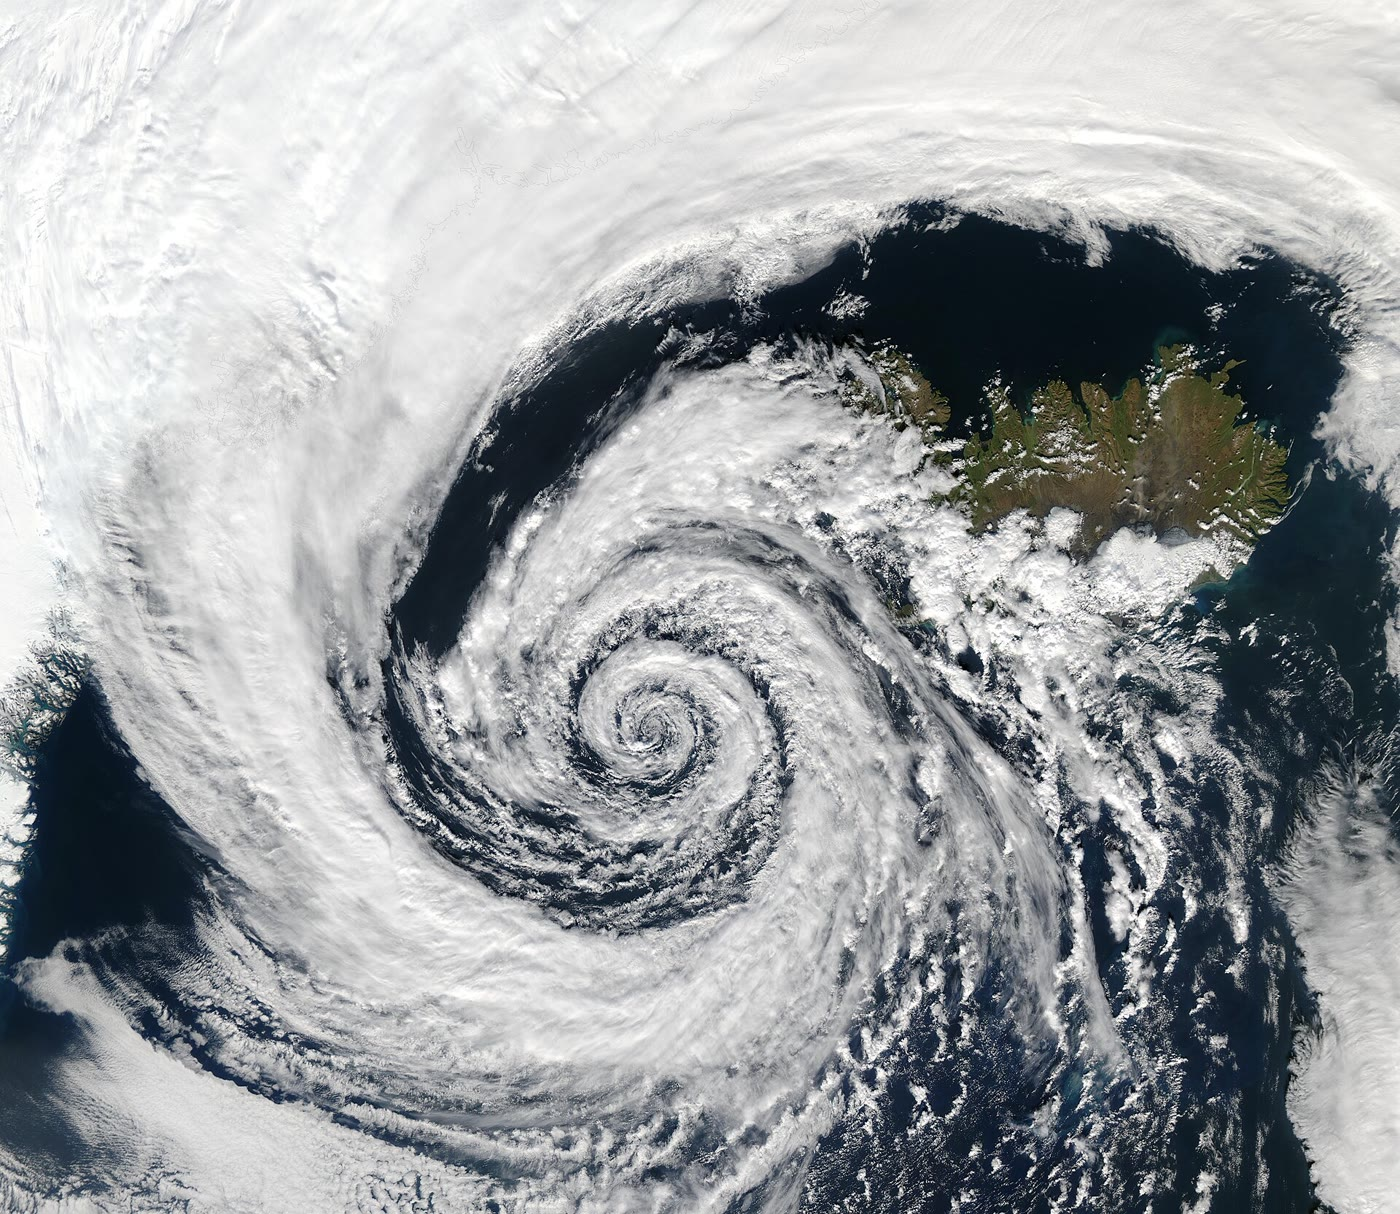
\includegraphics[width=\linewidth]{images/book5/b3-iceland-low.jpg}
\end{minipage}

\par\smallskip{\small À esquerda, a taxa de crescimento de Eady em função do comprimento de
onda para o cisalhamento zonal médio de janeiro a \ang{45} N (NCEP--NCAR Reanalysis~1,
1991--2020), a estratificação média da troposfera e $H = \qty{11}{km}$:
não há crescimento abaixo de \qty{3200}{km}, e o crescimento mais rápido ocorre perto de \qty{4700}{km}. À direita, uma
depressão em seu estágio maduro ao largo da costa sudoeste da Islândia, em 4
de setembro de 2003, com suas nuvens enroladas em uma espiral anti-horária ao redor do
centro de baixa pressão (NASA/GSFC, MODIS Rapid Response Team, domínio
público).}\label{fig:b3:atmospheric-dynamics:eady}
\end{omfigure}
% ledger: data:b5-ncep-uwnd, nasa:grc-atmos, photo:b3-iceland-low

O ciclone extratropical do volume do segundo ano é a face superficial de uma
onda baroclínica em crescimento: seu setor quente transporta ar quente para os polos e
para cima, o ar frio atrás dele desliza rumo ao equador e para baixo, e o cavado
em altitude inclina-se para oeste com a altura, como exige a liberação de
\omterm{def:b3:atmospheric-dynamics:ape}{energia potencial disponível}.

\section{A circulação geral}\label{sec:b3:atmospheric-dynamics:general-circulation}

A circulação geral é descrita pela média ao longo dos círculos de latitude,
e o que a média deixa de fora é tão importante quanto o que ela preserva.

\begin{definition}[Média zonal e turbilhões]\label{def:b3:atmospheric-dynamics:eddy}
A \emph{média zonal}\index{média zonal} de uma grandeza $A$ é sua média
ao longo de um círculo de latitude em altura ou pressão fixas, $[A] =
(1/2\pi)\int_0^{2\pi} A\,\mathrm d\lambda$. O desvio $A^* = A - [A]$
é sua parte de turbilhão; um \emph{turbilhão}\index{turbilhão (atmosférico)} da
atmosfera é qualquer desvio do escoamento em relação à sua média zonal: ondas migratórias,
ondas estacionárias, ciclones e anticiclones.
\end{definition}

A \omterm{def:b3:atmospheric-dynamics:eddy}{média zonal} de um produto divide-se em duas parcelas: $[vT] = [v][T] + [v^*T^*]$. O
primeiro termo é o transporte pela circulação meridional média, as células
do volume do primeiro ano; a segunda, o transporte pelos turbilhões. Nas
latitudes médias o vento meridional médio é fraco e o termo dos turbilhões
domina: o ar que se desloca para os polos é mais quente do que o ar que se desloca para o equador, na
mesma latitude, como mostra a figura abaixo, e $[v^*T^*] > 0$. Os turbilhões também
transportam momento de oeste, $[u^*v^*]$, dos subtrópicos para as latitudes
da corrente de jato, razão pela qual a corrente de jato e os ventos de oeste junto ao solo são
mantidos contra o atrito. A célula de Ferrel do volume do primeiro ano é a
circulação meridional média que esse transporte pelos turbilhões força.

\begin{omfigure}
\begin{tikzpicture}[>=stealth, font=\small, declare function={s(\x)=0.9*sin(\x r); t(\x)=0.9*sin((\x+1.0) r);}]
\draw[thick, black, domain=0:12.566, samples=120] plot (\x, {s(\x)});
\draw[omThm, thick, densely dashed, domain=0:12.566, samples=120] plot (\x, {t(\x)-0.15});
\foreach \x in {0.3, 6.58} {\draw[->, omThm, very thick] (\x,-1.1) -- (\x,1.15)
  node[above, font=\scriptsize] {quente};}
\foreach \x in {3.45, 9.73} {\draw[->, omDef, very thick] (\x,1.1) -- (\x,-1.15)
  node[below, font=\scriptsize] {frio};}
\node[font=\scriptsize, anchor=west, align=left] at (12.7,{s(12.566)}) {linha de\\corrente};
\node[font=\scriptsize, anchor=west, omThm] at (12.7,{t(12.566)-0.15}) {isoterma};
\draw[->] (-1.6,-1.1) -- (-0.6,-1.1) node[below, font=\scriptsize] {L};
\draw[->] (-1.6,-1.1) -- (-1.6,-0.1) node[above, font=\scriptsize] {N};
\node[font=\scriptsize] at (6.3,-1.95) {ar frio ao N, quente ao S};
\end{tikzpicture}

\par\smallskip{\small Onda baroclínica em crescimento, em planta (esquema,
Hemisfério Norte, escoamento de oeste). A isoterma (tracejada) atrasa-se em relação à
linha de corrente em um quarto de comprimento de onda ou menos, de modo que o ar que se desloca para o norte (setas
vermelhas) é mais quente do que o ar que se desloca para o sul na mesma latitude (azul):
a onda transporta calor para os polos, $[v^*T^*] >
0$.}\label{fig:b3:atmospheric-dynamics:heatflux}
\end{omfigure}

Nos trópicos os turbilhões são fracos e a circulação média transporta calor
para os polos, a célula de Hadley. O volume do primeiro ano mostrou que o ar que deixa o
equador em repouso, conservando seu momento angular, sopraria a centenas de
metros por segundo a \ang{40}, e deixou em aberto por que a célula termina perto de
\ang{30}. Um modelo simples responde.

\begin{definition}[Momento angular atmosférico; modelo de Held--Hou]\label{def:b3:atmospheric-dynamics:held-hou}
O \emph{momento angular atmosférico}\index{momento angular atmosférico}
por unidade de massa em torno do eixo da Terra é $M = (\Omega a\cos\varphi +
u)\,a\cos\varphi$, para um vento para leste $u$ na latitude $\varphi$. O
\emph{modelo de Held--Hou}\index{modelo de Held--Hou} da célula de Hadley é uma
circulação axissimétrica e estacionária de uma atmosfera seca de Boussinesq de profundidade
$H$, aquecida por relaxação em direção a uma temperatura potencial
de equilíbrio radiativo $\theta_E/\theta_0 = 1 + \Delta/3 - \Delta\sin^2\varphi$; seu
ramo superior conserva $M$, o ramo inferior tem vento desprezível, e o
escoamento obedece ao equilíbrio do \omterm{thm:b3:gfd-foundations:thermal-wind}{vento térmico}.
\end{definition}

\begin{theorem}[Extensão da célula de Hadley]\label{thm:b3:atmospheric-dynamics:held-hou}
No limite de ângulos pequenos, a célula de Held--Hou alcança a latitude
\[
\varphi_H = \left(\frac{5\,gH\Delta}{3\,\Omega^2a^2}\right)^{1/2}
\]
em cada hemisfério, e o vento de seu ramo superior é $u_M = \Omega
a\varphi^2$.
\end{theorem}

\begin{proof}
Para $\varphi$ pequeno, $\cos\varphi \approx 1$ e o ar que deixa o equador em
repouso com $M = \Omega a^2$ tem $u_M = \Omega a(1 - \cos^2\varphi)/\cos\varphi
\approx \Omega a\varphi^2$. Com $f \approx 2\Omega\varphi$, $y = a\varphi$,
vento nulo junto ao solo, e o \omterm{thm:b3:gfd-foundations:thermal-wind}{vento térmico}, em sua forma de Boussinesq, sobre a
profundidade $H$, $2\Omega\varphi\,u_M/H = -(g/a\theta_0)\,\partial\theta_M/
\partial\varphi$, em que $\theta_M$ é a média vertical de $\theta$ na
célula. Então $\partial(\theta_M/\theta_0)/\partial\varphi = -2\Omega^2a^2
\varphi^3/(gH)$ e $\theta_M/\theta_0 = A - K\varphi^4$, $K = \Omega^2a^2/
(2gH)$. Dentro da célula a circulação move calor, mas nem cria nem
destrói, de modo que a célula tem a mesma temperatura média que o equilíbrio
radiativo: $\int_0^{\varphi_H}\theta_M\,\mathrm d\varphi = \int_0^{\varphi_H}
\theta_E\,\mathrm d\varphi$. Na borda a temperatura é contínua:
$\theta_M(\varphi_H) = \theta_E(\varphi_H)$. Com $\theta_E/\theta_0 \approx
B - \Delta\varphi^2$, $B = 1 + \Delta/3$, a primeira condição dá $A - B =
K\varphi_H^4/5 - \Delta\varphi_H^2/3$, a segunda $A - B = K\varphi_H^4 -
\Delta\varphi_H^2$. Subtraindo, $(4/5)K\varphi_H^4 = (2/3)\Delta
\varphi_H^2$, logo $\varphi_H^2 = 5\Delta/(6K) = 5gH\Delta/(3\Omega^2a^2)$.
\end{proof}

A célula termina onde a temperatura imposta pela conservação do momento angular
encontra o equilíbrio radiativo; para além dela, a atmosfera teria de
estar mais fria do que a radiação a deixa. O modelo tem dois parâmetros que não são
observados diretamente. Para $H = \qty{15}{km}$ e $\Delta$ entre $1/6$ e
$1/3$, escolhido para ilustração, $\varphi_H$ fica entre \ang{25} e \ang{35}. As
células observadas, lidas a partir do vento meridional da \omterm{def:b3:atmospheric-dynamics:eddy}{média zonal}, terminam em
\ang{33.3} N e \ang{32.5} S na média anual, e as células de inverno,
as mais intensas, em \ang{30.8} N em dezembro--fevereiro e \ang{29.1} S em
junho--agosto. O essencial é a escala: uma célula que se alarga com uma
troposfera mais profunda e um contraste de aquecimento mais forte, e se estreita em um
planeta que gira mais depressa. O vento superior do modelo, $u_M =
\qty{88}{m/s}$ na borda para $\Delta = 1/6$, é o dobro do jato observado:
os turbilhões levam embora o excesso.
% ledger: geod5:grs80-defining, earth:Rmean, data:b5-ncep-vwnd (values in figdata/bachelor-3/held_hou.py)

\begin{omfigure}
\begin{tikzpicture}
\begin{groupplot}[group style={group size=2 by 1, horizontal sep=1.7cm},
  width=0.48\linewidth, height=0.44\linewidth, tick label style={font=\scriptsize},
  label style={font=\small}, legend style={font=\scriptsize, draw=none, fill=none}]
\nextgroupplot[xlabel={latitude (\unit{\degree})}, ylabel={$100\,(\theta/\theta_0 - 1)$},
  xmin=0, xmax=60, ymin=-30, ymax=15, legend pos=south west, legend cell align=left,
  title={\small $\Delta = 1/3$, $H = \qty{15}{km}$}]
% computed in figdata/bachelor-3/held_hou.py
\addplot[omDef, thick] table[x=phi, y=thE] {figdata/out/bachelor-3-held_hou-theta-3.dat};
\addplot[omThm, thick, unbounded coords=jump] table[x=phi, y=thM] {figdata/out/bachelor-3-held_hou-theta-3.dat};
\addplot[black!50, densely dashed, forget plot] coordinates {(35.26,-30) (35.26,15)};
\node[font=\scriptsize, anchor=south west] at (axis cs:35.6,7) {$\varphi_H$};
\legend{$\theta_E$, $\theta_M$}
\nextgroupplot[xlabel={latitude (\unit{\degree})}, ylabel={$\psi$ em \qty{500}{hPa} ($10^{10}$\,\unit{kg/s})},
  xmin=-60, xmax=60, ymin=-25, ymax=25, xtick={-60,-30,0,30,60}, legend pos=south west,
  legend cell align=left]
\addplot[black!50, thin, domain=-60:60, samples=2, forget plot] {0};
\addplot[black, thick] table[x=lat, y=ann] {figdata/out/bachelor-3-held_hou-psi.dat};
\addplot[omDef, thick] table[x=lat, y=djf] {figdata/out/bachelor-3-held_hou-psi.dat};
\addplot[omThm, thick] table[x=lat, y=jja] {figdata/out/bachelor-3-held_hou-psi.dat};
\legend{ano, dez--fev, jun--ago}
\end{groupplot}
\end{tikzpicture}

\par\smallskip{\small Esquerda, a construção de Held--Hou: a
temperatura da célula que conserva o momento angular (vermelho) encontra o
equilíbrio radiativo (azul) em $\varphi_H = \ang{35}$, com áreas iguais entre as
curvas dentro da célula. À direita, a função de corrente meridional de massa média em
\qty{500}{hPa} a partir do vento meridional da \omterm{def:b3:atmospheric-dynamics:eddy}{média zonal} (NCEP--NCAR
Reanalysis~1, 1991--2020; positiva onde o ar acima de \qty{500}{hPa}
se desloca para o norte): a forte
célula do hemisfério de inverno cruza o equador, e as células terminam perto de
\ang{30}.}\label{fig:b3:atmospheric-dynamics:held-hou}
\end{omfigure}
% ledger: data:b5-ncep-vwnd

\begin{history}[Das ondas longas à primeira previsão computada]
Em 1939, C.-G.~Rossby e seus colaboradores, no \emph{Journal of Marine
Research}, propuseram-se a interpretar vários fenômenos aparentemente independentes
do tempo a partir de um único ponto de vista. Motivado por padrões meteorológicos
que se deslocam a montante contra o escoamento predominante de oeste, Rossby formulou
uma teoria linearizada na qual perturbações de grande escala tendem a se deslocar para oeste
e as menores para leste em relação ao vento: as ondas e o
plano $\beta$ deste capítulo. Onze anos depois, J.~G.~Charney,
R.~Fjørtoft e J.~von~Neumann integraram a \omterm{thm:b3:atmospheric-dynamics:bve}{equação da vorticidade barotrópica}
numericamente no computador eletrônico ENIAC: quatro previsões de 24~horas no
nível de \qty{500}{mb}, em uma malha de \qty{736}{km}, 8 graus de longitude
em \ang{45}. O cálculo de cada previsão levou cerca de 24~horas: eles
estavam, como escreveram, apenas em condições de acompanhar o tempo.
\end{history}
% ledger: rossby39:paper, jmr20:commentary, charney50:eniac

\section{Exercícios}

\begin{exercise}[$\star$]\label{exo:b3:atmospheric-dynamics:1}
(a)~Calcule a \omterm{def:b3:atmospheric-dynamics:vorticity-kinds}{vorticidade relativa} de um vórtice em rotação de corpo rígido que dá
uma volta por dia. (b)~Calcule a \omterm{def:b3:atmospheric-dynamics:vorticity-kinds}{vorticidade planetária} em \ang{30} e \ang{60} N
($\Omega = \qty{7.292e-5}{rad/s}$) e compare.
\end{exercise}

\begin{exercise}[$\star$]\label{exo:b3:atmospheric-dynamics:2}
Uma parcela sem \omterm{def:b3:atmospheric-dynamics:vorticity-kinds}{vorticidade relativa} em \ang{30} N move-se para \ang{40} N em um
escoamento sem divergência. Calcule sua \omterm{def:b3:atmospheric-dynamics:vorticity-kinds}{vorticidade relativa} ali. Ela é
ciclônica ou anticiclônica?
\end{exercise}

\begin{exercise}[$\star$]\label{exo:b3:atmospheric-dynamics:3}
Em \ang{45} N, sem vento médio, calcule a velocidade de fase de uma onda de Rossby
de comprimento de onda \qty{5000}{km} com $l = 0$. Em que direção ela se desloca?
\end{exercise}

\begin{exercise}[$\star$]\label{exo:b3:atmospheric-dynamics:4}
Em \ang{60} N, com um vento de oeste de \qty{10}{m/s}, calcule $\beta$, o
comprimento de onda estacionário e o número de ondas estacionárias ao redor do
círculo de latitude ($a = \qty{6371}{km}$).
\end{exercise}

\begin{exercise}[$\star\star$]\label{exo:b3:atmospheric-dynamics:5}
Uma coluna de ar de \qty{10}{km} de profundidade, sem \omterm{def:b3:atmospheric-dynamics:vorticity-kinds}{vorticidade relativa} em \ang{45}
N, atravessa uma cadeia de montanhas que a comprime até \qty{8}{km}, e em seguida uma bacia
onde ela tem \qty{12}{km} de profundidade. Supondo que ela permaneça próxima de \ang{45} N, calcule sua
\omterm{def:b3:atmospheric-dynamics:vorticity-kinds}{vorticidade relativa} sobre a cadeia e sobre a bacia. Onde
as depressões tenderão a se formar?
\end{exercise}

\begin{exercise}[$\star\star$]\label{exo:b3:atmospheric-dynamics:6}
Para a onda com cinco cristas ao redor do círculo de \ang{45} N ($l = 0$) em um
vento de oeste de \qty{15}{m/s}, calcule a velocidade de fase e a velocidade de grupo.
Quanto tempo a energia da onda leva para percorrer \qty{5000}{km} para leste, e quanto
tempo leva o padrão?
\end{exercise}

\begin{exercise}[$\star\star$]\label{exo:b3:atmospheric-dynamics:7}
Em \ang{45} N, com um vento de oeste de \qty{15}{m/s}, uma onda fica confinada entre
latitudes de modo que $l = \pi/(\qty{6000}{km})$. (a)~Calcule seu número de onda zonal estacionário e seu
comprimento de onda. (b)~Mostre que nenhuma onda estacionária existe para
$l = \pi/(\qty{3000}{km})$.
\end{exercise}

\begin{exercise}[$\star\star$]\label{exo:b3:atmospheric-dynamics:8}
Em um \omterm{def:b3:atmospheric-dynamics:eady}{modelo de Eady} em \ang{45} N, $\Lambda = \qty{2e-3}{s^{-1}}$, $N =
\qty{0.012}{s^{-1}}$ e $H = \qty{10}{km}$. Calcule $L_d$, a taxa de crescimento
e o tempo de $e$-folding da perturbação de crescimento mais rápido, e seu
comprimento de onda.
\end{exercise}

\begin{exercise}[$\star\star$]\label{exo:b3:atmospheric-dynamics:9}
Ao longo de um círculo de latitude, o vento meridional do \omterm{def:b3:atmospheric-dynamics:eddy}{turbilhão} é $v^* = V\cos kx$ e a
temperatura do \omterm{def:b3:atmospheric-dynamics:eddy}{turbilhão} $T^* = T_0\cos(kx - \delta)$, com $V = \qty{10}{m/s}$ e
$T_0 = \qty{5}{K}$. Calcule $[v^*T^*]$ para $\delta = 0$, \ang{60} e
\ang{90}, e o fluxo de calor correspondente $\rho c_p[v^*T^*]$ por
\unit{kg/m^3} de ar ($c_p = \qty{1004}{J.kg^{-1}.K^{-1}}$). Qual
arranjo não transporta calor?
\end{exercise}

\begin{exercise}[$\star\star\star$]\label{exo:b3:atmospheric-dynamics:10}
Partindo da \omterm{thm:b3:atmospheric-dynamics:bve}{equação da vorticidade barotrópica}, deduza a \omterm{thm:b3:atmospheric-dynamics:rossby}{relação de dispersão
das ondas de Rossby} em um vento de oeste uniforme e mostre que, em relação
ao ar, toda onda de Rossby se desloca para oeste.
\end{exercise}

\begin{exercise}[$\star\star\star$]\label{exo:b3:atmospheric-dynamics:11}
No \omterm{def:b3:atmospheric-dynamics:held-hou}{modelo de Held--Hou}, tome $H = \qty{12}{km}$ e $\Delta = 1/4$. Calcule
$\varphi_H$, o vento de pequeno ângulo $u_M$ na borda e o vento exato de momento angular
nesse ponto, e compare com a corrente de jato subtropical de
\qty{44}{m/s} da \omterm{def:b3:atmospheric-dynamics:eddy}{média zonal} de janeiro.
\end{exercise}

\begin{exercise}[$\star\star\star$]\label{exo:b3:atmospheric-dynamics:12}
Duas camadas de ar diferem em temperatura potencial de \qty{10}{K} sobre \qty{300}{K};
a interface entre elas sobe em direção ao polo com inclinação $s$
ao longo de uma faixa de \qty{4000}{km} de largura, e $\rho = \qty{0.7}{kg/m^3}$. (a)~Mostre
que o achatamento da interface libera $\rho g' s^2L^2/24$ por unidade
de área, com $g' = g\,\Delta\theta/\theta$. (b)~Calcule essa energia para $s = 10^{-3}$ e
$2\times10^{-3}$ e compare-a com a energia cinética de um vento de \qty{15}{m/s}
através de \qty{10}{km} do mesmo ar.
\end{exercise}
% ledger: geod5:grs80-defining, earth:Rmean, data:b5-ncep-uwnd

\section{Problema: A onda que ficou parada}

\begin{problem}[{Problema de fim de semana --- vorticidade, ondas de Rossby e o
crescimento de uma onda baroclínica a \ang{45} N}]
\label{pb:b3:atmospheric-dynamics:1}
Um escoamento de oeste de \qty{15}{m/s} atravessa as latitudes médias de um
continente fictício, ao longo de \ang{45} N. Tome $\Omega =
\qty{7.292115e-5}{rad/s}$, $a = \qty{6371}{km}$ e $g = \qty{9.81}{m/s^2}$.
Todos os valores do escoamento são fictícios.

\medskip\noindent\textbf{Parte I --- Uma parcela deslocada.}
\begin{enumerate}
\item Uma parcela sem \omterm{def:b3:atmospheric-dynamics:vorticity-kinds}{vorticidade relativa} a \ang{45} N é empurrada para
  \ang{50} N. Calcule $f$ nas duas latitudes e sua \omterm{def:b3:atmospheric-dynamics:vorticity-kinds}{vorticidade relativa} a
  \ang{50} N, se o escoamento não tiver divergência.
\item Movendo-se com \qty{15}{m/s}, ao longo de qual raio de curvatura ela gira
  (tome $\zeta = -V/R$, toda ela devida à curvatura)? Para que lado ela gira?
\item Se sua coluna também se contrai de \qty{10.0}{km} para \qty{9.5}{km} ao longo do
  percurso, qual é sua \omterm{def:b3:atmospheric-dynamics:vorticity-kinds}{vorticidade relativa} a \ang{50} N?
\item Se for empurrada, em vez disso, para \ang{40} N, sem divergência, qual
  \omterm{def:b3:atmospheric-dynamics:vorticity-kinds}{vorticidade relativa} ela adquire? Explique por que uma parcela deslocada de sua
  latitude oscila em torno dela.
\end{enumerate}

\medskip\noindent\textbf{Parte II --- Ondas viajantes.}
\begin{enumerate}[resume]
\item Calcule $\beta$ a \ang{45} N e o comprimento do círculo de latitude.
\item Para $n = 3$ a 8 ondas ao longo do círculo ($l = 0$), calcule o
  comprimento de onda, a velocidade de fase e a velocidade de grupo nos ventos de oeste de
  \qty{15}{m/s}.
\item Quais ondas se deslocam para oeste, quais para leste? Quantos dias leva a onda
  $n = 5$ para percorrer \qty{1000}{km}?
\item Uma crista sobre o oeste do continente se intensifica. Onde, e após quanto
  tempo, o efeito da onda $n = 6$ alcançará \qty{5000}{km}
  a jusante?
\end{enumerate}

\medskip\noindent\textbf{Parte III --- A onda que ficou parada.}
\begin{enumerate}[resume]
\item Calcule o comprimento de onda estacionário e o número de onda estacionário a
  \ang{45} N.
\item Calcule o número de onda estacionário para ventos de oeste de 10 e
  \qty{20}{m/s}. O que acontece com as ondas estacionárias quando os ventos de oeste
  se intensificam no inverno?
\item Calcule o número de onda estacionário a \ang{35} N e \ang{55} N com
  ventos de oeste de \qty{15}{m/s}.
\item As montanhas do oeste do continente elevam-se \qty{2}{km} em uma
  troposfera de \qty{10}{km} de espessura. Calcule a \omterm{def:b3:atmospheric-dynamics:vorticity-kinds}{vorticidade relativa} de uma coluna
  que as atravessa sem mudar de latitude. Por que montanhas forçam
  ondas estacionárias?
\item Por que o padrão de ondas que as montanhas forçam permanece parado
  somente quando seu comprimento de onda está próximo de $\lambda_s$?
\end{enumerate}

\medskip\noindent\textbf{Parte IV --- Uma tempestade se intensifica.}
\begin{enumerate}[resume]
\item Os ventos de oeste aumentam da superfície até \qty{10}{km} em
  \qty{25}{m/s}. Calcule o cisalhamento $\Lambda$ e o gradiente de temperatura
  em direção ao polo que ele implica pelo \omterm{thm:b3:gfd-foundations:thermal-wind}{vento térmico}, a uma temperatura média de
  \qty{250}{K}.
\item Com $N = \qty{0.011}{s^{-1}}$, calcule o número de Richardson
  $N^2/\Lambda^2$. O escoamento é instável à turbulência de cisalhamento em pequena escala?
\item Calcule o raio de Rossby $L_d$ para $H = \qty{10}{km}$.
\item Calcule o comprimento de onda da perturbação de Eady de crescimento mais rápido e
  o número dessas ondas ao longo do círculo de latitude.
\item Calcule o menor comprimento de onda que cresce.
\item Calcule a taxa de crescimento $\sigma_{\max}$.
\item De que fator a perturbação cresce em três dias?
\item Compare o comprimento de onda da tempestade em crescimento com o
  comprimento de onda estacionário da Parte~III: qual é maior e o que isso implica para o
  movimento das tempestades em relação às ondas estacionárias?
\item Para que lado o cavado da onda em crescimento se inclina com a altura, e
  por que precisa fazê-lo?
\item Dê o tempo de $e$-folding da perturbação de Eady de crescimento mais rápido.
\end{enumerate}
\end{problem}
% ledger: geod5:grs80-defining, earth:Rmean
